\documentclass[border=10pt]{standalone}
\usepackage[svgnames]{xcolor}
\usepackage{amsmath}
\usepackage{pgfplots}
\pgfplotsset{compat=newest}
\usepackage[sfdefault]{FiraSans}
\usepackage{FiraMono}
\renewcommand*\familydefault{\sfdefault}
\begin{document}
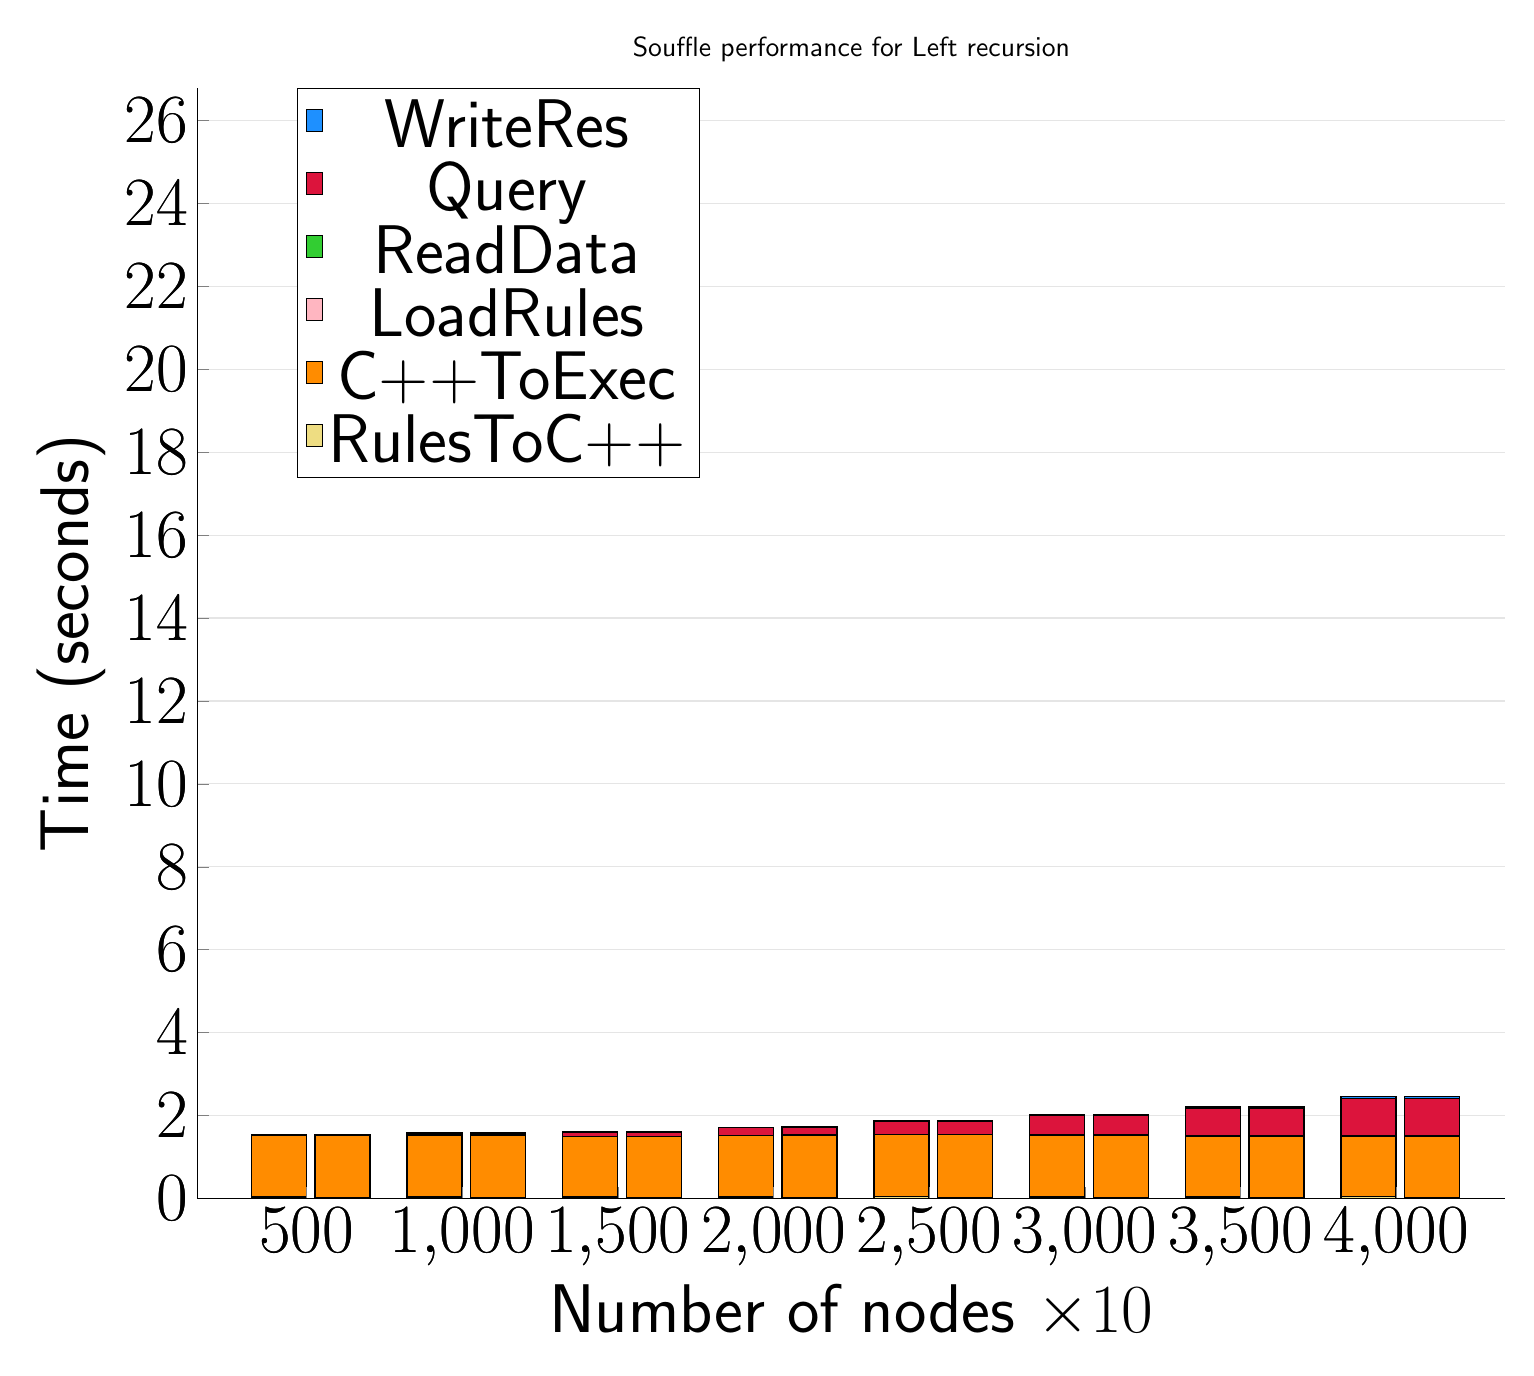
\begin{tikzpicture}
	\begin{axis}[
			ybar stacked,
			title={Souffle performance for Left recursion},
			bar shift=-10pt,
			width=1.5\textwidth,
			bar width=0.7cm,
			ymajorgrids, tick align=inside,
			major grid style={draw=gray!20},
			xtick=data,
			ymin=0, ymax=26.78465,
			axis x line*=bottom,
			axis y line*=left,
			enlarge x limits=0.1,
			legend style={
					at={(0.23, 1)},
					anchor=north,
					legend columns=1,
					font=\Huge,
				},
			ylabel={Time (seconds)},
			xlabel={Number of nodes $\times 10$},
			label style={font=\Huge},
			tick label style={font=\Huge},
		]
		\addlegendimage{fill=DodgerBlue, draw=black, line width=0.2pt}
		\addlegendentry{WriteRes}
		\addlegendimage{fill=Crimson, draw=black, line width=0.2pt}
		\addlegendentry{Query}
		\addlegendimage{fill=LimeGreen, draw=black, line width=0.2pt}
		\addlegendentry{ReadData}
		\addlegendimage{fill=LightPink, draw=black, line width=0.2pt}
		\addlegendentry{LoadRules}
		\addlegendimage{fill=DarkOrange, draw=black, line width=0.2pt}
		\addlegendentry{C++ToExec}
		\addlegendimage{fill=LightGoldenrod, draw=black, line width=0.2pt}
		\addlegendentry{RulesToC++}
		\addplot +[fill=LightGoldenrod, draw=black, line width=0.5pt] coordinates {
				(500, 0.04000003337860107)
				(1000, 0.04000005722045898)
				(1500, 0.04000005722045898)
				(2000, 0.04000003337860107)
				(2500, 0.04299995899200439)
				(3000, 0.04200000762939453)
				(3500, 0.04200000762939453)
				(4000, 0.043000006675720216)
			};
		\addplot +[fill=DarkOrange, draw=black, line width=0.5pt] coordinates {
				(500, 1.4829999923706054)
				(1000, 1.4900000095367432)
				(1500, 1.4549999713897706)
				(2000, 1.4789999961853026)
				(2500, 1.497000026702881)
				(3000, 1.4880000352859497)
				(3500, 1.4670000076293945)
				(4000, 1.4680000066757202)
			};
		\addplot +[fill=LightPink, draw=black, line width=0.5pt] coordinates {
				(500, 9.61709e-05)
				(1000, 0.00011190399999999999)
				(1500, 7.572919999999999e-05)
				(2000, 9.58458e-05)
				(2500, 7.85835e-05)
				(3000, 0.0001049333)
				(3500, 0.0001236914)
				(4000, 0.00010926669999999999)
			};
		\addplot +[fill=LimeGreen, draw=black, line width=0.5pt] coordinates {
				(500, 0.0013743770000000002)
				(1000, 0.002642487)
				(1500, 0.003730224)
				(2000, 0.0047855499999999995)
				(2500, 0.005410018999999999)
				(3000, 0.00709177)
				(3500, 0.008899403)
				(4000, 0.009880533)
			};
		\addplot +[fill=Crimson, draw=black, line width=0.5pt] coordinates {
				(500, 0.012807610000000002)
				(1000, 0.0450217)
				(1500, 0.10277707)
				(2000, 0.1848658)
				(2500, 0.3186834)
				(3000, 0.4617330999999999)
				(3500, 0.6649731999999999)
				(4000, 0.8902228999999998)
			};
		\addplot +[fill=DodgerBlue, draw=black, line width=0.5pt] coordinates {
				(500, 0.0011198115999999998)
				(1000, 0.0029939799999999994)
				(1500, 0.006575346)
				(2000, 0.011548720000000002)
				(2500, 0.017891370000000004)
				(3000, 0.025696759999999996)
				(3500, 0.03453304)
				(4000, 0.045140959999999994)
			};
	\end{axis}
	\begin{axis}[
			ybar stacked,
			bar shift=13pt,
			width=1.5\textwidth,
			bar width=0.7cm,
			ymajorgrids, tick align=inside,
			major grid style={draw=none},
			xtick=data,
			ymin=0, ymax=26.78465,
			axis x line*=none,
			axis y line*=none,
			enlarge x limits=0.1,
			label style={font=\Huge},
			tick label style={font=\Huge},
		]
		\addplot +[fill=LightGoldenrod, draw=black, line width=0.5pt] coordinates {
				(500, 0.030000000000000006)
				(1000, 0.030000000000000006)
				(1500, 0.030000000000000006)
				(2000, 0.030000000000000006)
				(2500, 0.030000000000000006)
				(3000, 0.030000000000000006)
				(3500, 0.030000000000000006)
				(4000, 0.030000000000000006)
			};
		\addplot +[fill=DarkOrange, draw=black, line width=0.5pt] coordinates {
				(500, 1.499)
				(1000, 1.499)
				(1500, 1.4700000000000002)
				(2000, 1.498)
				(2500, 1.5110000000000001)
				(3000, 1.502)
				(3500, 1.479)
				(4000, 1.482)
			};
		\addplot +[fill=LightPink, draw=black, line width=0.5pt] coordinates {
				(500, 9.549999999999999e-05)
				(1000, 0.0001109)
				(1500, 7.55e-05)
				(2000, 9.52e-05)
				(2500, 7.819999999999999e-05)
				(3000, 0.00010410000000000001)
				(3500, 0.0001227)
				(4000, 0.000108)
			};
		\addplot +[fill=LimeGreen, draw=black, line width=0.5pt] coordinates {
				(500, 0.0013733)
				(1000, 0.0026395)
				(1500, 0.0037284000000000006)
				(2000, 0.0047845)
				(2500, 0.0054067)
				(3000, 0.0070896)
				(3500, 0.0088945)
				(4000, 0.0098764)
			};
		\addplot +[fill=Crimson, draw=black, line width=0.5pt] coordinates {
				(500, 0.012786199999999998)
				(1000, 0.044885800000000003)
				(1500, 0.1024462)
				(2000, 0.1844246)
				(2500, 0.31751310000000005)
				(3000, 0.46051449999999994)
				(3500, 0.6629084000000001)
				(4000, 0.8883324)
			};
		\addplot +[fill=DodgerBlue, draw=black, line width=0.5pt] coordinates {
				(500, 0.0011163999999999998)
				(1000, 0.0029163)
				(1500, 0.0063707)
				(2000, 0.0113031)
				(2500, 0.017820500000000003)
				(3000, 0.025337600000000005)
				(3500, 0.034159100000000005)
				(4000, 0.0449107)
			};
	\end{axis}
\end{tikzpicture}

\end{document}
